\documentclass[twoside]{book}

% Packages required by doxygen
\usepackage{fixltx2e}
\usepackage{calc}
\usepackage{doxygen}
\usepackage[export]{adjustbox} % also loads graphicx
\usepackage{graphicx}
\usepackage[utf8]{inputenc}
\usepackage{makeidx}
\usepackage{multicol}
\usepackage{multirow}
\PassOptionsToPackage{warn}{textcomp}
\usepackage{textcomp}
\usepackage[nointegrals]{wasysym}
\usepackage[table]{xcolor}

% Font selection
\usepackage[T1]{fontenc}
\usepackage[scaled=.90]{helvet}
\usepackage{courier}
\usepackage{amssymb}
\usepackage{sectsty}
\renewcommand{\familydefault}{\sfdefault}
\allsectionsfont{%
  \fontseries{bc}\selectfont%
  \color{darkgray}%
}
\renewcommand{\DoxyLabelFont}{%
  \fontseries{bc}\selectfont%
  \color{darkgray}%
}
\newcommand{\+}{\discretionary{\mbox{\scriptsize$\hookleftarrow$}}{}{}}

% Page & text layout
\usepackage{geometry}
\geometry{%
  a4paper,%
  top=2.5cm,%
  bottom=2.5cm,%
  left=2.5cm,%
  right=2.5cm%
}
\tolerance=750
\hfuzz=15pt
\hbadness=750
\setlength{\emergencystretch}{15pt}
\setlength{\parindent}{0cm}
\setlength{\parskip}{3ex plus 2ex minus 2ex}
\makeatletter
\renewcommand{\paragraph}{%
  \@startsection{paragraph}{4}{0ex}{-1.0ex}{1.0ex}{%
    \normalfont\normalsize\bfseries\SS@parafont%
  }%
}
\renewcommand{\subparagraph}{%
  \@startsection{subparagraph}{5}{0ex}{-1.0ex}{1.0ex}{%
    \normalfont\normalsize\bfseries\SS@subparafont%
  }%
}
\makeatother

% Headers & footers
\usepackage{fancyhdr}
\pagestyle{fancyplain}
\fancyhead[LE]{\fancyplain{}{\bfseries\thepage}}
\fancyhead[CE]{\fancyplain{}{}}
\fancyhead[RE]{\fancyplain{}{\bfseries\leftmark}}
\fancyhead[LO]{\fancyplain{}{\bfseries\rightmark}}
\fancyhead[CO]{\fancyplain{}{}}
\fancyhead[RO]{\fancyplain{}{\bfseries\thepage}}
\fancyfoot[LE]{\fancyplain{}{}}
\fancyfoot[CE]{\fancyplain{}{}}
\fancyfoot[RE]{\fancyplain{}{\bfseries\scriptsize Generated by Doxygen }}
\fancyfoot[LO]{\fancyplain{}{\bfseries\scriptsize Generated by Doxygen }}
\fancyfoot[CO]{\fancyplain{}{}}
\fancyfoot[RO]{\fancyplain{}{}}
\renewcommand{\footrulewidth}{0.4pt}
\renewcommand{\chaptermark}[1]{%
  \markboth{#1}{}%
}
\renewcommand{\sectionmark}[1]{%
  \markright{\thesection\ #1}%
}

% Indices & bibliography
\usepackage{natbib}
\usepackage[titles]{tocloft}
\setcounter{tocdepth}{3}
\setcounter{secnumdepth}{5}
\makeindex

% Hyperlinks (required, but should be loaded last)
\usepackage{ifpdf}
\ifpdf
  \usepackage[pdftex,pagebackref=true]{hyperref}
\else
  \usepackage[ps2pdf,pagebackref=true]{hyperref}
\fi
\hypersetup{%
  colorlinks=true,%
  linkcolor=blue,%
  citecolor=blue,%
  unicode%
}

% Custom commands
\newcommand{\clearemptydoublepage}{%
  \newpage{\pagestyle{empty}\cleardoublepage}%
}

\usepackage{caption}
\captionsetup{labelsep=space,justification=centering,font={bf},singlelinecheck=off,skip=4pt,position=top}

%===== C O N T E N T S =====

\begin{document}

% Titlepage & ToC
\hypersetup{pageanchor=false,
             bookmarksnumbered=true,
             pdfencoding=unicode
            }
\pagenumbering{roman}
\begin{titlepage}
\vspace*{7cm}
\begin{center}%
{\Large T\+P1\+\_\+c }\\
\vspace*{1cm}
{\large Generated by Doxygen 1.8.11}\\
\end{center}
\end{titlepage}
\clearemptydoublepage
\tableofcontents
\clearemptydoublepage
\pagenumbering{arabic}
\hypersetup{pageanchor=true}

%--- Begin generated contents ---
\chapter{Data Structure Index}
\section{Data Structures}
Here are the data structures with brief descriptions\+:\begin{DoxyCompactList}
\item\contentsline{section}{\hyperlink{structTLex}{T\+Lex} \\*Structure contenant tous les parametres/donnees pour l\textquotesingle{}analyse lexicale }{\pageref{structTLex}}{}
\item\contentsline{section}{\hyperlink{structTSymbole}{T\+Symbole} \\*Union permettant de manipuler un entier/reel/chaine pour la table des symboles }{\pageref{structTSymbole}}{}
\end{DoxyCompactList}

\chapter{File Index}
\section{File List}
Here is a list of all documented files with brief descriptions\+:\begin{DoxyCompactList}
\item\contentsline{section}{\hyperlink{paramcmdl_8c}{paramcmdl.\+c} \\*Contient le code des fonctions }{\pageref{paramcmdl_8c}}{}
\item\contentsline{section}{\hyperlink{paramcmdl_8h}{paramcmdl.\+h} \\*Contient les prototypes des fonctions }{\pageref{paramcmdl_8h}}{}
\item\contentsline{section}{\hyperlink{tp1__c_8c}{tp1\+\_\+c.\+c} \\*Contient la fonction main }{\pageref{tp1__c_8c}}{}
\end{DoxyCompactList}

\chapter{Data Structure Documentation}
\hypertarget{structTParamDef}{}\section{T\+Param\+Def Struct Reference}
\label{structTParamDef}\index{T\+Param\+Def@{T\+Param\+Def}}


represente un parametre de la ligne de commande (nom,type,valeur...)  




Collaboration diagram for T\+Param\+Def\+:\nopagebreak
\begin{figure}[H]
\begin{center}
\leavevmode
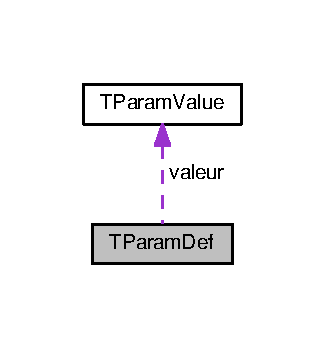
\includegraphics[width=156pt]{structTParamDef__coll__graph}
\end{center}
\end{figure}
\subsection*{Data Fields}
\begin{DoxyCompactItemize}
\item 
char $\ast$ \hyperlink{structTParamDef_afa78db012abc7fecd18c60d6154e04f8}{nom}
\item 
\hyperlink{paramcmdl_8c_a07d4e5a29d675892ddc5f377533c06a5}{T\+Param\+Type} \hyperlink{structTParamDef_aaa8c69f39c6dd02a968dc15044810327}{type}
\item 
char \hyperlink{structTParamDef_a66254f6368c5542d3f14afdd1ea1e621}{lettre}
\item 
\hyperlink{unionTParamValue}{T\+Param\+Value} \hyperlink{structTParamDef_a3f5cbf75e393d35bb230dfe293f7c7ba}{valeur}
\end{DoxyCompactItemize}


\subsection{Detailed Description}
represente un parametre de la ligne de commande (nom,type,valeur...) 

\subsection{Field Documentation}
\index{T\+Param\+Def@{T\+Param\+Def}!lettre@{lettre}}
\index{lettre@{lettre}!T\+Param\+Def@{T\+Param\+Def}}
\subsubsection[{\texorpdfstring{lettre}{lettre}}]{\setlength{\rightskip}{0pt plus 5cm}char T\+Param\+Def\+::lettre}\hypertarget{structTParamDef_a66254f6368c5542d3f14afdd1ea1e621}{}\label{structTParamDef_a66254f6368c5542d3f14afdd1ea1e621}
lettre a utiliser sur la ligne de commande \index{T\+Param\+Def@{T\+Param\+Def}!nom@{nom}}
\index{nom@{nom}!T\+Param\+Def@{T\+Param\+Def}}
\subsubsection[{\texorpdfstring{nom}{nom}}]{\setlength{\rightskip}{0pt plus 5cm}char$\ast$ T\+Param\+Def\+::nom}\hypertarget{structTParamDef_afa78db012abc7fecd18c60d6154e04f8}{}\label{structTParamDef_afa78db012abc7fecd18c60d6154e04f8}
nom du parametre \index{T\+Param\+Def@{T\+Param\+Def}!type@{type}}
\index{type@{type}!T\+Param\+Def@{T\+Param\+Def}}
\subsubsection[{\texorpdfstring{type}{type}}]{\setlength{\rightskip}{0pt plus 5cm}{\bf T\+Param\+Type} T\+Param\+Def\+::type}\hypertarget{structTParamDef_aaa8c69f39c6dd02a968dc15044810327}{}\label{structTParamDef_aaa8c69f39c6dd02a968dc15044810327}
type (entier,reel,chaine) \index{T\+Param\+Def@{T\+Param\+Def}!valeur@{valeur}}
\index{valeur@{valeur}!T\+Param\+Def@{T\+Param\+Def}}
\subsubsection[{\texorpdfstring{valeur}{valeur}}]{\setlength{\rightskip}{0pt plus 5cm}{\bf T\+Param\+Value} T\+Param\+Def\+::valeur}\hypertarget{structTParamDef_a3f5cbf75e393d35bb230dfe293f7c7ba}{}\label{structTParamDef_a3f5cbf75e393d35bb230dfe293f7c7ba}
valeur a affecter au parametre 

The documentation for this struct was generated from the following file\+:\begin{DoxyCompactItemize}
\item 
\hyperlink{paramcmdl_8c}{paramcmdl.\+c}\end{DoxyCompactItemize}

\hypertarget{unionTParamValue}{}\section{T\+Param\+Value Union Reference}
\label{unionTParamValue}\index{T\+Param\+Value@{T\+Param\+Value}}


union permettant de manipuler un entier/reel/chaine  


\subsection*{Data Fields}
\begin{DoxyCompactItemize}
\item 
int {\bfseries entier}\hypertarget{unionTParamValue_a85a2847d254115d744ac7d55391dc1ea}{}\label{unionTParamValue_a85a2847d254115d744ac7d55391dc1ea}

\item 
float {\bfseries reel}\hypertarget{unionTParamValue_a6c6e99a421de592ad46cf47aab9cef58}{}\label{unionTParamValue_a6c6e99a421de592ad46cf47aab9cef58}

\item 
const char $\ast$ {\bfseries chaine}\hypertarget{unionTParamValue_a3e12f31017e3dd1bb79801330f767a22}{}\label{unionTParamValue_a3e12f31017e3dd1bb79801330f767a22}

\end{DoxyCompactItemize}


\subsection{Detailed Description}
union permettant de manipuler un entier/reel/chaine 

The documentation for this union was generated from the following file\+:\begin{DoxyCompactItemize}
\item 
\hyperlink{paramcmdl_8c}{paramcmdl.\+c}\end{DoxyCompactItemize}

\chapter{File Documentation}
\hypertarget{paramcmdl_8c}{}\section{paramcmdl.\+c File Reference}
\label{paramcmdl_8c}\index{paramcmdl.\+c@{paramcmdl.\+c}}


Contient le code des fonctions.  


{\ttfamily \#include $<$stdio.\+h$>$}\\*
{\ttfamily \#include $<$string.\+h$>$}\\*
{\ttfamily \#include $<$ctype.\+h$>$}\\*
{\ttfamily \#include $<$stdlib.\+h$>$}\\*
Include dependency graph for paramcmdl.\+c\+:\nopagebreak
\begin{figure}[H]
\begin{center}
\leavevmode
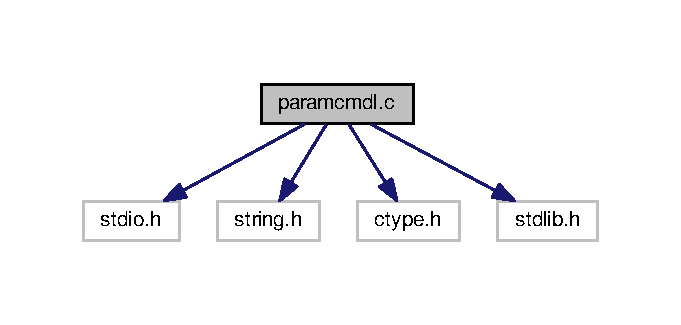
\includegraphics[width=327pt]{paramcmdl_8c__incl}
\end{center}
\end{figure}
This graph shows which files directly or indirectly include this file\+:
\nopagebreak
\begin{figure}[H]
\begin{center}
\leavevmode
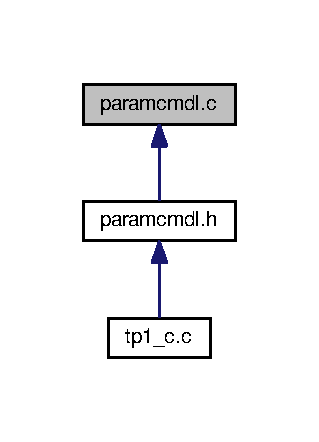
\includegraphics[width=153pt]{paramcmdl_8c__dep__incl}
\end{center}
\end{figure}
\subsection*{Data Structures}
\begin{DoxyCompactItemize}
\item 
union \hyperlink{unionTParamValue}{T\+Param\+Value}
\begin{DoxyCompactList}\small\item\em union permettant de manipuler un entier/reel/chaine \end{DoxyCompactList}\item 
struct \hyperlink{structTParamDef}{T\+Param\+Def}
\begin{DoxyCompactList}\small\item\em represente un parametre de la ligne de commande (nom,type,valeur...) \end{DoxyCompactList}\end{DoxyCompactItemize}
\subsection*{Enumerations}
\begin{DoxyCompactItemize}
\item 
enum \hyperlink{paramcmdl_8c_a07d4e5a29d675892ddc5f377533c06a5}{T\+Param\+Type} \{ \hyperlink{paramcmdl_8c_a07d4e5a29d675892ddc5f377533c06a5a8d6edc98669af667cc9e31340845978a}{P\+Tentier}, 
\hyperlink{paramcmdl_8c_a07d4e5a29d675892ddc5f377533c06a5aea24482a7d983b9b03681bb4bb45be09}{P\+Treel}, 
\hyperlink{paramcmdl_8c_a07d4e5a29d675892ddc5f377533c06a5abd88632411744fe81117441047cb065a}{P\+Tchaine}
 \}\begin{DoxyCompactList}\small\item\em Constantes pour le type des parametres de la ligne de commande. \end{DoxyCompactList}
\end{DoxyCompactItemize}
\subsection*{Functions}
\begin{DoxyCompactItemize}
\item 
char $\ast$ \hyperlink{paramcmdl_8c_a7ebf667ae7249e66ffc7ed75ed38e13d}{Valeur\+Param\+To\+String} (\hyperlink{structTParamDef}{T\+Param\+Def} $\ast$\+\_\+tab\+Param, const int \+\_\+index)
\begin{DoxyCompactList}\small\item\em fonction qui transforme la valeur d\textquotesingle{}un parametre en chaine de caractere \end{DoxyCompactList}\item 
void \hyperlink{paramcmdl_8c_a43aaeaf65d8f18907fd5abc1e1c40209}{Print\+Param} (\hyperlink{structTParamDef}{T\+Param\+Def} $\ast$\+\_\+tab\+Param, const int \+\_\+nb\+Param)
\begin{DoxyCompactList}\small\item\em fonction qui affiche a l\textquotesingle{}ecran les parametre, leur type et leur valeur \end{DoxyCompactList}\item 
int \hyperlink{paramcmdl_8c_a9468b57ddf26450a9adb40b155fb1c16}{Read\+Param\+From\+Command\+Line} (\hyperlink{structTParamDef}{T\+Param\+Def} $\ast$\+\_\+tab\+Param, const int \+\_\+nb\+Param, const int \+\_\+argc, const char $\ast$\+\_\+argv\mbox{[}$\,$\mbox{]})
\begin{DoxyCompactList}\small\item\em fonction qui analyse la ligne de commande pour en extraire des valeurs pour les parametres \end{DoxyCompactList}\end{DoxyCompactItemize}
\subsection*{Variables}
\begin{DoxyCompactItemize}
\item 
char $\ast$ \hyperlink{paramcmdl_8c_a45f6ef32ea85374f1fccef0bf09dd548}{Param\+Type\+Chaine} \mbox{[}$\,$\mbox{]} = \{\char`\"{}entier\char`\"{},\char`\"{}reel\char`\"{},\char`\"{}chaine\char`\"{}\}
\end{DoxyCompactItemize}


\subsection{Detailed Description}
Contient le code des fonctions. 

\begin{DoxyAuthor}{Author}
NM 

Pierrick B\+O\+B\+ET 

Rémy B\+O\+U\+T\+E\+L\+O\+UP 
\end{DoxyAuthor}
\begin{DoxyVersion}{Version}
0.\+1 
\end{DoxyVersion}
\begin{DoxyDate}{Date}
06/12/2016 
\end{DoxyDate}


\subsection{Enumeration Type Documentation}
\index{paramcmdl.\+c@{paramcmdl.\+c}!T\+Param\+Type@{T\+Param\+Type}}
\index{T\+Param\+Type@{T\+Param\+Type}!paramcmdl.\+c@{paramcmdl.\+c}}
\subsubsection[{\texorpdfstring{T\+Param\+Type}{TParamType}}]{\setlength{\rightskip}{0pt plus 5cm}enum {\bf T\+Param\+Type}}\hypertarget{paramcmdl_8c_a07d4e5a29d675892ddc5f377533c06a5}{}\label{paramcmdl_8c_a07d4e5a29d675892ddc5f377533c06a5}


Constantes pour le type des parametres de la ligne de commande. 

\begin{Desc}
\item[Enumerator]\par
\begin{description}
\index{P\+Tentier@{P\+Tentier}!paramcmdl.\+c@{paramcmdl.\+c}}\index{paramcmdl.\+c@{paramcmdl.\+c}!P\+Tentier@{P\+Tentier}}\item[{\em 
P\+Tentier\hypertarget{paramcmdl_8c_a07d4e5a29d675892ddc5f377533c06a5a8d6edc98669af667cc9e31340845978a}{}\label{paramcmdl_8c_a07d4e5a29d675892ddc5f377533c06a5a8d6edc98669af667cc9e31340845978a}
}]un nombre entier \index{P\+Treel@{P\+Treel}!paramcmdl.\+c@{paramcmdl.\+c}}\index{paramcmdl.\+c@{paramcmdl.\+c}!P\+Treel@{P\+Treel}}\item[{\em 
P\+Treel\hypertarget{paramcmdl_8c_a07d4e5a29d675892ddc5f377533c06a5aea24482a7d983b9b03681bb4bb45be09}{}\label{paramcmdl_8c_a07d4e5a29d675892ddc5f377533c06a5aea24482a7d983b9b03681bb4bb45be09}
}]un nombre reel \index{P\+Tchaine@{P\+Tchaine}!paramcmdl.\+c@{paramcmdl.\+c}}\index{paramcmdl.\+c@{paramcmdl.\+c}!P\+Tchaine@{P\+Tchaine}}\item[{\em 
P\+Tchaine\hypertarget{paramcmdl_8c_a07d4e5a29d675892ddc5f377533c06a5abd88632411744fe81117441047cb065a}{}\label{paramcmdl_8c_a07d4e5a29d675892ddc5f377533c06a5abd88632411744fe81117441047cb065a}
}]une chaine de caracteres \end{description}
\end{Desc}


\subsection{Function Documentation}
\index{paramcmdl.\+c@{paramcmdl.\+c}!Print\+Param@{Print\+Param}}
\index{Print\+Param@{Print\+Param}!paramcmdl.\+c@{paramcmdl.\+c}}
\subsubsection[{\texorpdfstring{Print\+Param(\+T\+Param\+Def $\ast$\+\_\+tab\+Param, const int \+\_\+nb\+Param)}{PrintParam(TParamDef *_tabParam, const int _nbParam)}}]{\setlength{\rightskip}{0pt plus 5cm}Print\+Param (
\begin{DoxyParamCaption}
\item[{{\bf T\+Param\+Def} $\ast$}]{\+\_\+tab\+Param, }
\item[{const int}]{\+\_\+nb\+Param}
\end{DoxyParamCaption}
)}\hypertarget{paramcmdl_8c_a43aaeaf65d8f18907fd5abc1e1c40209}{}\label{paramcmdl_8c_a43aaeaf65d8f18907fd5abc1e1c40209}


fonction qui affiche a l\textquotesingle{}ecran les parametre, leur type et leur valeur 


\begin{DoxyParams}[1]{Parameters}
\mbox{\tt in}  & {\em \+\_\+tab\+Param} & tableau des parametres de la ligne de commande \\
\hline
\mbox{\tt in}  & {\em \+\_\+nb\+Param} & taille du tableau \\
\hline
\end{DoxyParams}
\begin{DoxyReturn}{Returns}
neant 
\end{DoxyReturn}
Affichage des valeurs du paramètre serveur

Affichage des valeurs du paramètre appli

Affichage des valeurs du paramètre tours \index{paramcmdl.\+c@{paramcmdl.\+c}!Read\+Param\+From\+Command\+Line@{Read\+Param\+From\+Command\+Line}}
\index{Read\+Param\+From\+Command\+Line@{Read\+Param\+From\+Command\+Line}!paramcmdl.\+c@{paramcmdl.\+c}}
\subsubsection[{\texorpdfstring{Read\+Param\+From\+Command\+Line(\+T\+Param\+Def $\ast$\+\_\+tab\+Param, const int \+\_\+nb\+Param, const int \+\_\+argc, const char $\ast$\+\_\+argv[])}{ReadParamFromCommandLine(TParamDef *_tabParam, const int _nbParam, const int _argc, const char *_argv[])}}]{\setlength{\rightskip}{0pt plus 5cm}int Read\+Param\+From\+Command\+Line (
\begin{DoxyParamCaption}
\item[{{\bf T\+Param\+Def} $\ast$}]{\+\_\+tab\+Param, }
\item[{const int}]{\+\_\+nb\+Param, }
\item[{const int}]{\+\_\+argc, }
\item[{const char $\ast$}]{\+\_\+argv\mbox{[}$\,$\mbox{]}}
\end{DoxyParamCaption}
)}\hypertarget{paramcmdl_8c_a9468b57ddf26450a9adb40b155fb1c16}{}\label{paramcmdl_8c_a9468b57ddf26450a9adb40b155fb1c16}


fonction qui analyse la ligne de commande pour en extraire des valeurs pour les parametres 


\begin{DoxyParams}[1]{Parameters}
\mbox{\tt out}  & {\em \+\_\+tab\+Param} & tableau des parametres de la ligne de commande \\
\hline
\mbox{\tt in}  & {\em \+\_\+nb\+Param} & taille du tableau \\
\hline
\mbox{\tt in}  & {\em \+\_\+argc} & nombre d\textquotesingle{}arguments passes sur la ligne de commande \\
\hline
\mbox{\tt in}  & {\em \+\_\+argv} & tableau qui contient les chaines de caracteres passees en arguments du programme \\
\hline
\end{DoxyParams}
\begin{DoxyReturn}{Returns}
$>$=0 \+: nombre de parametres mis a jour, $<$0 \+: erreur 
\end{DoxyReturn}
Recherche de la valeur -\/s dans les paramètres fournis

Si la valeur n\textquotesingle{}a pas été trouvé, une erreur est renvoyée

Affection des valeurs pour le paramètre serveur

Recherche de la valeur -\/a dans les paramètres fournis

Si la valeur n\textquotesingle{}a pas été trouvé, une erreur est renvoyée

Affection des valeurs pour le paramètre appli

Recherche de la valeur -\/t dans les paramètres fournis

Si la valeur n\textquotesingle{}a pas été trouvé, une erreur est renvoyée

Affection des valeurs pour le paramètre tours \index{paramcmdl.\+c@{paramcmdl.\+c}!Valeur\+Param\+To\+String@{Valeur\+Param\+To\+String}}
\index{Valeur\+Param\+To\+String@{Valeur\+Param\+To\+String}!paramcmdl.\+c@{paramcmdl.\+c}}
\subsubsection[{\texorpdfstring{Valeur\+Param\+To\+String(\+T\+Param\+Def $\ast$\+\_\+tab\+Param, const int \+\_\+index)}{ValeurParamToString(TParamDef *_tabParam, const int _index)}}]{\setlength{\rightskip}{0pt plus 5cm}char $\ast$ Valeur\+Param\+To\+String (
\begin{DoxyParamCaption}
\item[{{\bf T\+Param\+Def} $\ast$}]{\+\_\+tab\+Param, }
\item[{const int}]{\+\_\+index}
\end{DoxyParamCaption}
)}\hypertarget{paramcmdl_8c_a7ebf667ae7249e66ffc7ed75ed38e13d}{}\label{paramcmdl_8c_a7ebf667ae7249e66ffc7ed75ed38e13d}


fonction qui transforme la valeur d\textquotesingle{}un parametre en chaine de caractere 


\begin{DoxyParams}[1]{Parameters}
\mbox{\tt in}  & {\em \+\_\+tab\+Param} & tableau des parametres de la ligne de commande \\
\hline
\mbox{\tt in}  & {\em \+\_\+index} & indice du parametre a considerer dans le tableau \\
\hline
\end{DoxyParams}
\begin{DoxyReturn}{Returns}
une nouvelle chaine (qu\textquotesingle{}il faudra libérer par la suite) 
\end{DoxyReturn}


\subsection{Variable Documentation}
\index{paramcmdl.\+c@{paramcmdl.\+c}!Param\+Type\+Chaine@{Param\+Type\+Chaine}}
\index{Param\+Type\+Chaine@{Param\+Type\+Chaine}!paramcmdl.\+c@{paramcmdl.\+c}}
\subsubsection[{\texorpdfstring{Param\+Type\+Chaine}{ParamTypeChaine}}]{\setlength{\rightskip}{0pt plus 5cm}char$\ast$ Param\+Type\+Chaine\mbox{[}$\,$\mbox{]} = \{\char`\"{}entier\char`\"{},\char`\"{}reel\char`\"{},\char`\"{}chaine\char`\"{}\}}\hypertarget{paramcmdl_8c_a45f6ef32ea85374f1fccef0bf09dd548}{}\label{paramcmdl_8c_a45f6ef32ea85374f1fccef0bf09dd548}
constante chaine de caracteres pour l\textquotesingle{}affichage des types 
\hypertarget{paramcmdl_8h}{}\section{paramcmdl.\+h File Reference}
\label{paramcmdl_8h}\index{paramcmdl.\+h@{paramcmdl.\+h}}


Contient les prototypes des fonctions.  


{\ttfamily \#include \char`\"{}paramcmdl.\+c\char`\"{}}\\*
Include dependency graph for paramcmdl.\+h\+:
\nopagebreak
\begin{figure}[H]
\begin{center}
\leavevmode
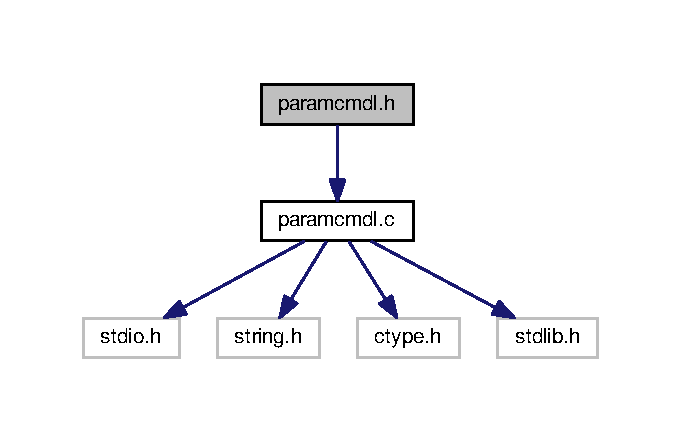
\includegraphics[width=327pt]{paramcmdl_8h__incl}
\end{center}
\end{figure}
This graph shows which files directly or indirectly include this file\+:
\nopagebreak
\begin{figure}[H]
\begin{center}
\leavevmode
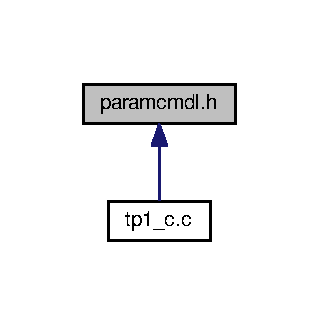
\includegraphics[width=153pt]{paramcmdl_8h__dep__incl}
\end{center}
\end{figure}
\subsection*{Functions}
\begin{DoxyCompactItemize}
\item 
char $\ast$ \hyperlink{paramcmdl_8h_a09f083d05cb2f8560fc6976719c7b443}{Valeur\+Param\+To\+String} (\hyperlink{structTParamDef}{T\+Param\+Def} $\ast$\+\_\+tab\+Param, const int \+\_\+index)
\begin{DoxyCompactList}\small\item\em fonction qui transforme la valeur d\textquotesingle{}un parametre en chaine de caractere \end{DoxyCompactList}\item 
void \hyperlink{paramcmdl_8h_a22d0708077876d73979d6880dc7bfe4d}{Print\+Param} (\hyperlink{structTParamDef}{T\+Param\+Def} $\ast$\+\_\+tab\+Param, const int \+\_\+nb\+Param)
\begin{DoxyCompactList}\small\item\em fonction qui affiche a l\textquotesingle{}ecran les parametre, leur type et leur valeur \end{DoxyCompactList}\item 
int \hyperlink{paramcmdl_8h_a9468b57ddf26450a9adb40b155fb1c16}{Read\+Param\+From\+Command\+Line} (\hyperlink{structTParamDef}{T\+Param\+Def} $\ast$\+\_\+tab\+Param, const int \+\_\+nb\+Param, const int \+\_\+argc, const char $\ast$\+\_\+argv\mbox{[}$\,$\mbox{]})
\begin{DoxyCompactList}\small\item\em fonction qui analyse la ligne de commande pour en extraire des valeurs pour les parametres \end{DoxyCompactList}\end{DoxyCompactItemize}


\subsection{Detailed Description}
Contient les prototypes des fonctions. 

\begin{DoxyAuthor}{Author}
NM 

Pierrick B\+O\+B\+ET 

Rémy B\+O\+U\+T\+E\+L\+O\+UP 
\end{DoxyAuthor}
\begin{DoxyVersion}{Version}
0.\+1 
\end{DoxyVersion}
\begin{DoxyDate}{Date}
06/12/2016 
\end{DoxyDate}


\subsection{Function Documentation}
\index{paramcmdl.\+h@{paramcmdl.\+h}!Print\+Param@{Print\+Param}}
\index{Print\+Param@{Print\+Param}!paramcmdl.\+h@{paramcmdl.\+h}}
\subsubsection[{\texorpdfstring{Print\+Param(\+T\+Param\+Def $\ast$\+\_\+tab\+Param, const int \+\_\+nb\+Param)}{PrintParam(TParamDef *_tabParam, const int _nbParam)}}]{\setlength{\rightskip}{0pt plus 5cm}void Print\+Param (
\begin{DoxyParamCaption}
\item[{{\bf T\+Param\+Def} $\ast$}]{\+\_\+tab\+Param, }
\item[{const int}]{\+\_\+nb\+Param}
\end{DoxyParamCaption}
)}\hypertarget{paramcmdl_8h_a22d0708077876d73979d6880dc7bfe4d}{}\label{paramcmdl_8h_a22d0708077876d73979d6880dc7bfe4d}


fonction qui affiche a l\textquotesingle{}ecran les parametre, leur type et leur valeur 


\begin{DoxyParams}[1]{Parameters}
\mbox{\tt in}  & {\em \+\_\+tab\+Param} & tableau des parametres de la ligne de commande \\
\hline
\mbox{\tt in}  & {\em \+\_\+nb\+Param} & taille du tableau \\
\hline
\end{DoxyParams}
\begin{DoxyReturn}{Returns}
neant 
\end{DoxyReturn}
Affichage des valeurs du paramètre serveur

Affichage des valeurs du paramètre appli

Affichage des valeurs du paramètre tours \index{paramcmdl.\+h@{paramcmdl.\+h}!Read\+Param\+From\+Command\+Line@{Read\+Param\+From\+Command\+Line}}
\index{Read\+Param\+From\+Command\+Line@{Read\+Param\+From\+Command\+Line}!paramcmdl.\+h@{paramcmdl.\+h}}
\subsubsection[{\texorpdfstring{Read\+Param\+From\+Command\+Line(\+T\+Param\+Def $\ast$\+\_\+tab\+Param, const int \+\_\+nb\+Param, const int \+\_\+argc, const char $\ast$\+\_\+argv[])}{ReadParamFromCommandLine(TParamDef *_tabParam, const int _nbParam, const int _argc, const char *_argv[])}}]{\setlength{\rightskip}{0pt plus 5cm}int Read\+Param\+From\+Command\+Line (
\begin{DoxyParamCaption}
\item[{{\bf T\+Param\+Def} $\ast$}]{\+\_\+tab\+Param, }
\item[{const int}]{\+\_\+nb\+Param, }
\item[{const int}]{\+\_\+argc, }
\item[{const char $\ast$}]{\+\_\+argv\mbox{[}$\,$\mbox{]}}
\end{DoxyParamCaption}
)}\hypertarget{paramcmdl_8h_a9468b57ddf26450a9adb40b155fb1c16}{}\label{paramcmdl_8h_a9468b57ddf26450a9adb40b155fb1c16}


fonction qui analyse la ligne de commande pour en extraire des valeurs pour les parametres 


\begin{DoxyParams}[1]{Parameters}
\mbox{\tt out}  & {\em \+\_\+tab\+Param} & tableau des parametres de la ligne de commande \\
\hline
\mbox{\tt in}  & {\em \+\_\+nb\+Param} & taille du tableau \\
\hline
\mbox{\tt in}  & {\em \+\_\+argc} & nombre d\textquotesingle{}arguments passes sur la ligne de commande \\
\hline
\mbox{\tt in}  & {\em \+\_\+argv} & tableau qui contient les chaines de caracteres passees en arguments du programme \\
\hline
\end{DoxyParams}
\begin{DoxyReturn}{Returns}
$>$=0 \+: nombre de parametres mis a jour, $<$0 \+: erreur 
\end{DoxyReturn}
Recherche de la valeur -\/s dans les paramètres fournis

Si la valeur n\textquotesingle{}a pas été trouvé, une erreur est renvoyée

Affection des valeurs pour le paramètre serveur

Recherche de la valeur -\/a dans les paramètres fournis

Si la valeur n\textquotesingle{}a pas été trouvé, une erreur est renvoyée

Affection des valeurs pour le paramètre appli

Recherche de la valeur -\/t dans les paramètres fournis

Si la valeur n\textquotesingle{}a pas été trouvé, une erreur est renvoyée

Affection des valeurs pour le paramètre tours \index{paramcmdl.\+h@{paramcmdl.\+h}!Valeur\+Param\+To\+String@{Valeur\+Param\+To\+String}}
\index{Valeur\+Param\+To\+String@{Valeur\+Param\+To\+String}!paramcmdl.\+h@{paramcmdl.\+h}}
\subsubsection[{\texorpdfstring{Valeur\+Param\+To\+String(\+T\+Param\+Def $\ast$\+\_\+tab\+Param, const int \+\_\+index)}{ValeurParamToString(TParamDef *_tabParam, const int _index)}}]{\setlength{\rightskip}{0pt plus 5cm}char$\ast$ Valeur\+Param\+To\+String (
\begin{DoxyParamCaption}
\item[{{\bf T\+Param\+Def} $\ast$}]{\+\_\+tab\+Param, }
\item[{const int}]{\+\_\+index}
\end{DoxyParamCaption}
)}\hypertarget{paramcmdl_8h_a09f083d05cb2f8560fc6976719c7b443}{}\label{paramcmdl_8h_a09f083d05cb2f8560fc6976719c7b443}


fonction qui transforme la valeur d\textquotesingle{}un parametre en chaine de caractere 


\begin{DoxyParams}[1]{Parameters}
\mbox{\tt in}  & {\em \+\_\+tab\+Param} & tableau des parametres de la ligne de commande \\
\hline
\mbox{\tt in}  & {\em \+\_\+index} & indice du parametre a considerer dans le tableau \\
\hline
\end{DoxyParams}
\begin{DoxyReturn}{Returns}
une nouvelle chaine (qu\textquotesingle{}il faudra libérer par la suite) 
\end{DoxyReturn}

\hypertarget{tp1__c_8c}{}\section{tp1\+\_\+c.\+c File Reference}
\label{tp1__c_8c}\index{tp1\+\_\+c.\+c@{tp1\+\_\+c.\+c}}


Contient la fonction main.  


{\ttfamily \#include \char`\"{}paramcmdl.\+h\char`\"{}}\\*
Include dependency graph for tp1\+\_\+c.\+c\+:
\nopagebreak
\begin{figure}[H]
\begin{center}
\leavevmode
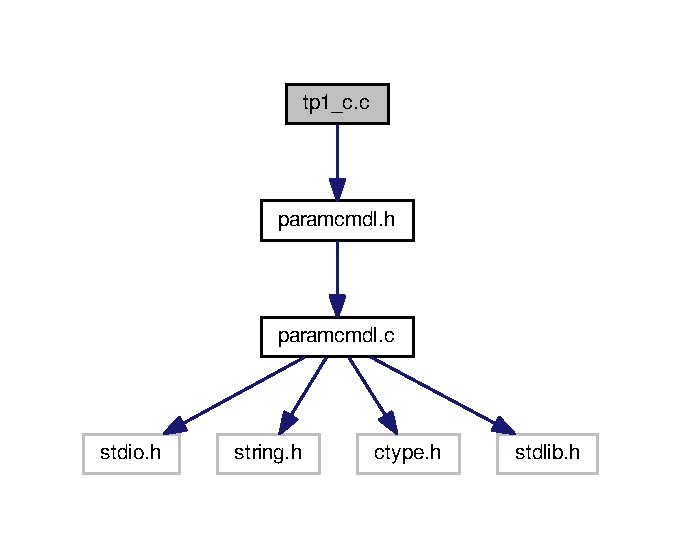
\includegraphics[width=327pt]{tp1__c_8c__incl}
\end{center}
\end{figure}
\subsection*{Functions}
\begin{DoxyCompactItemize}
\item 
int \hyperlink{tp1__c_8c_a065a3ee9a7ec43a06ab2fddbc3019a17}{main} (const int \+\_\+argc, const char $\ast$\+\_\+argv\mbox{[}$\,$\mbox{]})
\begin{DoxyCompactList}\small\item\em fonction principale \end{DoxyCompactList}\end{DoxyCompactItemize}


\subsection{Detailed Description}
Contient la fonction main. 

\begin{DoxyAuthor}{Author}
NM 

Pierrick B\+O\+B\+ET 

Rémy B\+O\+U\+T\+E\+L\+O\+UP 
\end{DoxyAuthor}
\begin{DoxyVersion}{Version}
0.\+1 
\end{DoxyVersion}
\begin{DoxyDate}{Date}
06/12/2016 
\end{DoxyDate}


\subsection{Function Documentation}
\index{tp1\+\_\+c.\+c@{tp1\+\_\+c.\+c}!main@{main}}
\index{main@{main}!tp1\+\_\+c.\+c@{tp1\+\_\+c.\+c}}
\subsubsection[{\texorpdfstring{main(const int \+\_\+argc, const char $\ast$\+\_\+argv[])}{main(const int _argc, const char *_argv[])}}]{\setlength{\rightskip}{0pt plus 5cm}int main (
\begin{DoxyParamCaption}
\item[{const int}]{\+\_\+argc, }
\item[{const char $\ast$}]{\+\_\+argv\mbox{[}$\,$\mbox{]}}
\end{DoxyParamCaption}
)}\hypertarget{tp1__c_8c_a065a3ee9a7ec43a06ab2fddbc3019a17}{}\label{tp1__c_8c_a065a3ee9a7ec43a06ab2fddbc3019a17}


fonction principale 


\begin{DoxyParams}[1]{Parameters}
\mbox{\tt in}  & {\em \+\_\+argc} & \+: nombre d\textquotesingle{}arguments passes sur la ligne de commande \\
\hline
\mbox{\tt in}  & {\em \+\_\+argv} & \+: tableau qui contient les chaines de caracteres passes en arguments du programme \\
\hline
\end{DoxyParams}
\begin{DoxyReturn}{Returns}
0 si terminaison normale 
\end{DoxyReturn}

%--- End generated contents ---

% Index
\backmatter
\newpage
\phantomsection
\clearemptydoublepage
\addcontentsline{toc}{chapter}{Index}
\printindex

\end{document}
